\chapter{\texorpdfstring{\MakeUppercase{Preston Royal Case Study}}{Preston Royal Case Study}}

Preston Royal Branch Library is a one-story building with \SI{12400}{\feet\squared} of gross floor area. The
library opened in 1954. The facility consists of an open-space reading room and circulation, staff
area, and an auditorium.

The library is served by a single air handling unit. A BAS graphic of
the AHU is shown in \figref{} \ref{fig:PrestonRoyalAHUGraphic}. 

The AHU has 14 terminal units that serve the various areas of the
library and are shown in \figref{} \ref{fig:PrestonRoyalAHUGraphic} and
\ref{fig:PrestonRoyalTerminalUnitLayout}.

The terminal units are parallel fan powered boxes. A BAS graphic of one
of the terminal units is shown in \figref{}
\ref{fig:PrestonRoyalTerminalUnitGraphic}.

\begin{figure}
\centering
\includegraphics[width=\textwidth]{Images/PrestonRoyalAHUGraphic.PNG}
\caption{Preston Royal AHU BAS Graphic.}
\label{fig:PrestonRoyalAHUGraphic}
\end{figure}

\begin{figure}
\centering
\includegraphics[width=\textwidth]{Images/PrestonRoyalFPBLayoutGraphic.PNG}
\caption{Preston Royal terminal unit layout.}
\label{fig:PrestonRoyalTerminalUnitLayout}
\end{figure}

\begin{figure}
\centering
\includegraphics[width=\textwidth]{Images/PrestonRoyalTerminalUnitGraphic.PNG}
\caption{Preston Royal terminal unit graphic. }
\label{fig:PrestonRoyalTerminalUnitGraphic}
\end{figure}



\section{Preston Royal Zone Load Analysis}

The zone load profile for Preston Royal showed similarities to the NCTM
building. During operation, the estimated zone load fluctuated up and
down throughout the day. \figref{}
\ref{fig:2017-04-03-1250-ZoneLoadforFPB02-TikzData} shows an example of
how the zone load cycles up and down many times per hour. Again, the
hypothesized explanation for this is not that the actual heat gain in
the space is fluctuating, but that the HVAC controls are oscillating. 

\begin{figure}
\centering
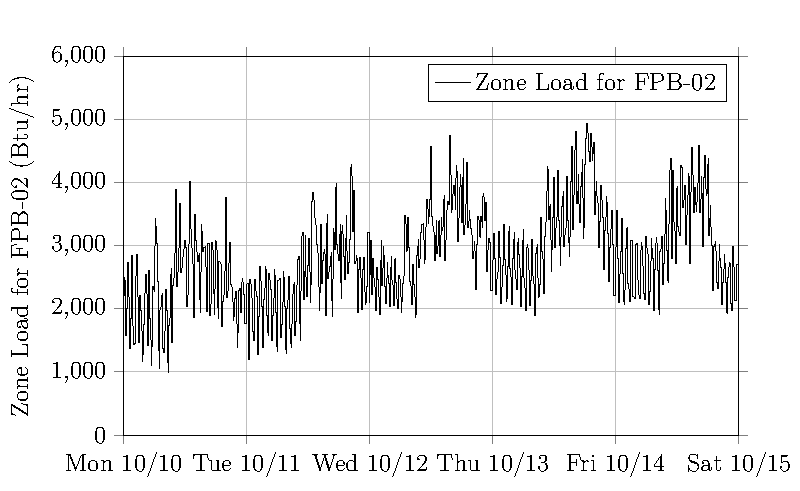
\includegraphics[]{Plots/2017-04-03-1250-ZoneLoadforFPB02-TikzData.pdf}
\caption{Zone load for FPB02 at Preston Royal Library.}
\label{fig:2017-04-03-1250-ZoneLoadforFPB02-TikzData}
\end{figure}
